\documentclass[12pt,a4paper]{article}
\usepackage[utf8]{inputenc}
\usepackage{amsmath}
\usepackage{amsthm}
\usepackage{amsfonts}
\usepackage{amssymb}
\usepackage[overload]{empheq}
\usepackage{color}
\usepackage[dvipsnames]{xcolor}
\usepackage{fullpage}
\usepackage{algorithm}
\usepackage{algpseudocode}
\usepackage{graphicx}

\title{PFSP heuristics project}

\author{Dorian Dumez}

\begin{document}
\maketitle

\section{Code}

\subsection{How to use}

The whole project can be compiled by making "make" in the code directory. Beside all .o file can be deleted with "make clean" in the same directory. Finally the main can be called on all instances with the script "multiple\_run.sh" at the root of this project, results are stoked in the "tmp.txt" file.\\

The main code call the tabu search and the iterative local search with given parameter on the given instance. The only two common parameter are the instance, specified with "--instance path\_to\_instance", and the time budget (always the same for the three function), specified with "--tmax time\_budget\_as\_long". Then the output will be de mean value over 5 execution (or 1 for deterministic algorithm) of the measurement. Score, relative deviation and execution time can be measured, this is chose by comment/uncomment preprocessor variable at the beginning of "main.cpp".

We can say that we have two tabu search, one with the exchange neighbourhood and one with the insert one, It's choose with the "--neighbourTabu neighbour\_index" (1 for exchange and 2 for insert). But these two tabu search use same parameter so the neighbourhood to use is just one of them. First, the tabu list length control the time that a move stay tabou, it's controlled with "--tabuListLenght integer\_value". Secondly, the long time memory impact is a floating point value that quantify the penalisation weight of the long time memory, it's controlled with "--longTimeMemoryImpact double\_value". Finally, the restart threshold is the acceptable relative deviation between the current solution and the best one, if this exceed the current solution become again the best one, this is set with "--restartThreshold double\_value".

Contrary to tabu search ILS have way more parameter. The first one is the same as tabu : the neighbourhood relation to use. It's choose with "neighbourILS neighbour\_index" (1 for transpose,2 for exchange,3 for insert, 4 and 5 for the two VND). All local search can be done in first or best improvement, controlled by "--DD boolean" (0 for first improvement and 1 for deepest descent). The third one is choice of the move used for perturbations, same as the first parameter it's "--neighbourPerturb neighbour\_index" (1 for exchange and 2 for insert). The next two are here to tune the perturbation procedure. perturbFrac is here to chose the fraction of the solution that should be change, use it with "--perturbFrac double\_beetween\_0\_and\_1". perturbRadius allow to limit the power of a perturbation by bounded it, it(s controlled with "--perturbRadius double\_beetween\_0\_and\_1" (0 allow only small perturbation and 1 all of them). Finally come the most parametrized choice : the acceptance criterion of new solution. It's control with "--acceptanceCrit index", where :
\begin{itemize}
\item
1 is for only improvement
\item
2 is for always
\item
3 is the metropolis, which need other parameter :
\begin{itemize}
\item
T0 the initial temperature, chose with "--T0 double"
\item
alpha the cooling factor, chose with "--alpha double"
\item
l the length of cooling plateau, chose with "--l long"
\item
warmupThreshold the lower bound of the temperature (if it's reach a warmup is used), chose with "--warmupThreshold double"
\item
T1 the temperature after a warmup, chose with "--T1 double", but according to \cite{Ruiz06asimple} (and M. Stuetzle advice) only $0.3, 0.6, 0.9, 1.2 \text{ and } 1.5$ are available
\end{itemize}
\item
4 is for the metropolis type proposed in \cite{Ruiz06asimple}. It's require a parameter lambda controlled with "--lambda double"
\end{itemize}

\subsection{Initial solution}

For all of following algorithm the initial solution is constructed with the rz heuristic. Indeed regarding to experiments we did in the first part a random initialisation hasn't any advantage over the rz heuristic. Beside in \cite{Pan201231} they use it too, so i look like a good initialisation.

\subsection{Tabu search}

For my tabu search I choose to use the exchange or the insert neighbourhood. Indeed they were best one in descent algorithm, beside in \cite{Tseng2010121} they use their tabu search with these neighbourhood.\\

In a tabu search the whole neighbourhood is crossed to search the best solution. But tabu movement, movement which have been done too recently, aren't checked. With the exchange a movement is the exchange of job at the index i and j. With insert it's move the job which was at the place i to the place j. Beside for both of them the movement is symmetric, i and j can be inverse without changing the modification, so the tabu list take care of that. To conclude the basis of our tabu search is to cross neighbourhood by selecting the best non-tabou neighbour (a neighbour which can be reach with a non-tabou movement) until the budget time is used.\\

Starting from this basic version I add some feature. They are inspired by my knowledge, the article of fred glover \cite{tabuprinciple} and a usage of a tabu search on the same problem in \cite{Tseng2010121}. But in \cite{Tseng2010121} they have slightly different usage of this algorithm because it's only the local of a genetic algorithm.

The first improvement of our tabu search is the well known aspiration criteria. Now we crossed the whole neighbourhood each time, and even test the tabou move. Then if the move give us access to a better solution than the best found so far this movement is keep. I mean that the tabou criteria can be ignored if a better solution than the best one is found. This move is so classic and logic that is not a parameter and it was included is our first iteration of the tabu search.

The second improvement is the long time memory. Indeed, because of the symmetric property of our move, we use only the half of the tabu matrix. I mean when we do a move we stock the next date (number of the iteration) when it will be available, so the tabu list data-structure is a $\text{nbJob} \times \text{nbJob}$ matrix of long (for the date). So we can use the other half of this matrix to count how many times a move have been done. Then the goal is to diversify the search so we penalised too used movement. I mean instead of just go to the neighbour which have the best value according to the evaluation function we go to the one which have the best evaluation. This evaluation is now $value(solution) + longTimeMemoryImpact*numberOfUsage(move)$, longTimeMemoryImpact is a parameter fixed by the user. Beside we can notice that this add on allow to avoid solution cycle (some can be longer than the tabu list length) by penalised move of these cycle. As a drawback if this factor is too hight their no intensification anymore.

The third improvement is the restart to the best so far. The goal of feature is to do more intensification in promising zone of the search space. Indeed during a tabu search we travel a lot across the solution space, so we might go into non interesting zone. Obviously we doesn't want to spend to much time with bad solution. Then the idea is when we go to a too bad solution we can think we are in a non-promising zone, because we always go the best solution in the neighbourhood (plus the small difference of the long time memory). In these case we want to go back in a promising zone as quickly as possible, so go back to the best solution found so far is a good way. Technically when we go to a solution which have a value superior to $(1 + \text{restartThreshold}) * value(best)$ the current solution become again this best solution. The restart threshold is a parameter given by the user. Contrary to the long time memory when this threshold is too low their no exploration, and even get out a local minima zone may be impossible.\\

After the first tuning session I notice that I can slightly modified the long time memory and the tabu list for the exchange neighbourhood to make it more meaningful. Basically a move was the exchange of two slots, the ith job and the jth one. But if we say that it's the exchange of the job at th ith place and the on at the jth place it's more logic. Because it's mean that the job A is before the job B or the contrary. First we can notice that it doesn't change anything with the tabu list, because they aren't move anyway. But it give a physical meaning to the long time memory : how many time we've tried A before B or B before A.

\subsection{ILS}

My IlS follow the basic outline of this algorithm \ref{outline ILS}, it's not wrote but we always keep track of the best solution found.

\begin{algorithm}
\caption{outline ILS}
\begin{algorithmic}[1]
\Procedure{ILS}{}
\State $s = \Call{Construction}$
\State $s = \Call{LocalSearch}{s}$
\While{EndCriterion}
	\State $s' = \Call{Perturb}{s}$
	\State $s' = \Call{LocalSearch}{s'}$
	\State $\textbf{If } \Call{Acceptable}{s'} \textbf{ Then } s = s'$
\EndWhile	
\EndProcedure
\end{algorithmic}
\label{outline ILS}
\end{algorithm}

For the same reason than before I always use the rz heuristic for construction. So their no option in the construction procedure.

The local search can be done with all option we seen in the first part of the project. Transpose is available because of is run time, indeed this allow to do a lot of local search, even if they should have a lower quality. All other are available because don't give that bad quality solution and aren't too slow, so I would like to test it. Beside all of these local search can be done in first or best improvement.

For the perturbation only exchange and insert are available, because transpose doesn't modify that much a solution. A perturbation will be random movement in these neighbourhood. Then a very important choice must be done : how much the solution should be change. We formalize that with the PerturbRatio, the ratio of job that is change (in fact a movement change 2 job so it's 2 times this ratio). So if it's 0 we don't perturb, so it's just a descent and the algorithm will be stick in the local minima during all the while loop. As contrary if it's 1 (or more than $0.5$) we do a complete restart every time, so there no intensification, beside as we seen in the first part random construction is quite bad. But if we take a balance ratio, for example 5\% (so 10\% of the job are move), we perturb enough to get out local minima but it's not a restart. Beside the local search become a bit faster, indeed the solution is already quite good so the convergence is faster. With this idea we can add an other parameter : PerturbRadius. The radius of perturbation restrict the perturbation by limited possible move. A perturbation move is allow only if the two random number aren't too spread, in the exchange neighbourhood that mean that the two exchanged job aren't too spread in the schedule and in the insert that the job isn't insert too far away from his current position in the schedule. In practice we take the first random number, $rnd1$, freely in $[\![ 0 , nbJob-1 ]\!]$ and the second one only in $[\![ rnd1 - nbJob*PerturbRadius -1 , rnd1 + nbJob*PerturbRadius +1 ]\!]$. So we have just $2*nbJob*PerturbRaduis +2$ choice for the second number, so if $PerturbRadius \leqslant 0.5 - \frac{1}{nbJob}$ it's a restriction of the possible perturbation. The $\pm 1$ is here as a security, in that way, even if PerturbRadius is too low related to the instance size, their always possible move. Same as PerturbRatio a small PerturbRaduis will encourage intensification with the risk that will stay stuck in a local minima, and a big one will encourage diversification. But we shall see them as a couple because their are strongly linked. Indeed they can be both balance to performed some movement which conserve the general shape of the solution. But they can be more exotic, for example a high PerturbRatio with a small PerturbRadius can work because it will do a lot small modification, so it's still conserve the shape of the solution.

Their also few possibility for the acceptance criterion, I mean the function which decide if the new solution become the current one. I take all possibility described in \cite{Pan201231} and I add the metropolis condition (the classical condition of simulated annealing) even if it's parameterfull. The first one is to keep the solution only if it's improve the current solution, so only if it's the new best. This choice completely kill diversification in favour of intensification, so it shall be counterbalance by perturbation. The second one, always accept, is the contrary. Because it always accept the new solution the perturbation shouldn’t change too much the solution to allow the algorithm to do a bit of intensification. The third one is the metropolis condition, this one can accept worst solution based on probability. This probability depend of the current temperature of the algorithm, which is closely related to the execution time. More formally $T = T_0 \times \alpha^{\lfloor date/l \rfloor}$ then the probability of keeping a degrading solution is $e^{ \frac{-\delta}{T}}$ where
\begin{itemize}
\item
$\delta$ is the value of the solution minus the value of the current solution
\item
date is the number of loop that had been performed
\item
$T_0$ is the initial temperature, passed as parameter
\item
l is the length of a cooling plateau, give as parameter
\item
$\alpha$ is the cooling factor, an other parameter
\end{itemize}
The value of $T_0$ should be quite high to allow the algorithm to escape the local minima basin of the first local search (which is quite good according to the first part). But in practice it should be found by experiment because it depend of the magnitude and the variation of the objective function. The value of l should be proportional to the size of the neighbourhood relation because it's related to the time we'll spend to cross it. But it's also should be determined by experiment because it depend of the landscape of the objective space. Finally $\alpha$ determined the time we give to the algorithm to converge. Classically this factor is quite high, over $0.8$, to give time to the algorithm and don't force him to converge in a bad local minima basin. But it shouldn't be too high or the algorithm will take a lot of time to converge, so maybe loose many time in bad region. With all of that we can notice that after a first convergence the algorithm stay stuck in his local minima, which may not be the global one. So a warm up strategy had been implemented, if the temperature go bellow a threshold we augment it. In practice if the temperature go bellow warmupThreshold we put it at the value $T_1$. Obviously $T_0 > T_1 > \text{warmupThreshold}$. More precisely the threshold should be quite low to allow the algorithm to do some intensification in promising zone, but it shouldn't be too low to avoid to spend too much time stuck in a local minima and reject all solution. Beside $T_1$ should be an average between $T_0$ and warmupThreshold because we neither want to restart the algorithm neither warm up to just move in our local minima basin without escape it. The previous criterion can be very efficient but it require a lot of parameter, all strongly linked, and their are closely linked to the instance type. So I add an other criterion, described in \cite{Ruiz06asimple}, as a compromise. In fact it's the metropolis criterion but with a constant temperature $\lambda \times \frac{\sum \limits_{i = 1}^{nbJob} \sum \limits_{j=1}^{nbMac} p_{ij} }{10 \times nbJob \times nbMac}$ where nbJob is the number of job, nbMac the number of machine and $\lambda$ a parameter. According to \cite{Pan201231} $\lambda$ is a robust parameter but according to \cite{Ruiz06asimple} it should be quite low. Finally M. Stuetzle advise me to test only some value : 0.3, 0.6, 0.9, 1.2 and 1.5.
 
\section{Tuning}

\subsection{Tabu search }

For the tuning of parameter I start by doing it myself by multiple try. Then I notice that these 3 parameter are strongly linked so they can't be study independently. And visualize at the same time 3 parameter is complicated so I just found a not too bad setting . But most important I feel extreme value of these one, out of them the feature become useless or destabilize to much the algorithm :
\begin{itemize}
\item
between $6$ and $17$ for the tabu list length, in \cite{Tseng2010121} they use 7 but with a restricted candidate list
\item
between $0.001$ and $1$ for the impact memory
\item
between $0.05$ and $0.4$ for the restart threshold
\end{itemize}
With slightly extend bound I run the irace algorithm \cite{irace}. Indeed I extend these bound to allow the algorithm to find exotic setting or to disable an incapacitating feature. It run during 20 hours (4800 run of the tabu search, on 3 core, forth one for the system) on my computer with size 50 instances. I chose to only use small instance because a run already need 45 seconds, $500 * 0.09$ (execution time of VND transpose $\rightarrow$ exchange $\rightarrow$ insert with rz heuristic) and I can't parallelyze more.\\

So i do the tuning run previously described twice : one time with the exchange neighbourhood and one time with the insert one. As say previously before I slightly modified the exchange version so I do an other training with irace. But this one was based on the result of the previous version so with an initial solution, smaller bound for parameter but also a smaller budget. Best setting output by irace are compiled in the table \ref{Setting of tabu search}.

\begin{table}[!h]
\centering
\begin{tabular}{|*{7}{c|}}
  \hline
  neighbourhood & tabu tenure & long time memory impact & restart threshold \\
  \hline
  exchange & $10$ & $0.001$ & $0.3$ \\ 
  exchange2 & $9$ & $0.26$ & $0.048$ \\
  insert & $15$ & $0.544$ & $0.061$ \\
  \hline
\end{tabular}
\caption{Setting of tabu search}
\label{Setting of tabu search}
\end{table}

We notice that setting with exchange neighbourhood (first iteration) are quite balance, but a bit centre on intensification. Indeed this combo of tabu tenure and long time memory impact allow some intensification but avoid cycling, and the restart threshold is not that hight so the algorithm will explore a bit but still based on intensification. The second iteration with exchange still quite balance but in the other way : the long time memory push to diversification and the restart on intensification. On the contrary setting output for insert neighbourhood are more exotic. Both tabu list and long time memory will really push to diversification (because associated parameter are very high), and the restart will take care of intensification. So it will act a bit like the second version of exchange but in a more exaggerated way.

\subsection{ILS}

Because of the huge amount of possible setting of ILS I just do one big run of irace. Indeed their is 80 combination of categorical parameter, plus some of them with real one. Beside all of the parameter can't be tested separated and their value compared by statistical test because many of them are strongly linked. So for this big run I give 10560 run (40h on 3 core) as budget. Beside I give to the algorithm quite good solution that I found by hand on few instances. Finally bounds on parameter had been used in the same way as the tabu race. Beside constraint on the value of $T_0$, $T_1$ and warmupThreshold had been add.\\

After the irace run I obtain the following parameter :
\begin{itemize}
\item
Local search : VND with transpose then exchange then insert (code $4$) in first improvement
\item
For the perturbation :
\begin{itemize}
\item
Insert neighbourhood
\item
Fraction of perturbation of $0.068$ (so $13.6 \%$ are modified)
\item
Radius of perturbation of $0.083$ (so with the size $50$ instances a radius of $4$)
\end{itemize}
\item
For the acceptance criterion :
\begin{itemize}
\item
Metropolis criterion
\item
$\alpha$ (the cooling factor) at $0.938$
\item
l (the plateau size) at $128$
\item
An initial temperature of $572$
\item
A warm up threshold of $24$ (reach after $6243$ iterations)
\item
A temperature after warm up of $1012$
\end{itemize}
\end{itemize}
First of all we notice an unexpected value of the temperature, for an unknown reason constraint on these two hadn't been taken in account by irace, and value it found are very curious. It will start by exploring the neighbourhood of the construct solution, and only after try something else. But finally by other experiment it appear that the algorithm do only around $900$ iterations, so irace disable the warm up by using a too low warm up threshold, so the warm up temperature doesn't matter anymore. Considering all of that this setting are relay based on intensification because we don't perturb that much and then use a powerful local search (so it may fall again in the same local minima) beside the acceptance criterion setting aren't that permissive.

\section{Analysis}

For all the test, all algorithm had been run on each instance. For tabu search only one time because both tabu and rz algorithm are deterministic. And because of the probability involve in ILS an average had been done over 5 run.\\
To cram table I use some abbreviation :
\begin{itemize}
\item
tabuE for the tabu search with exchange neighbourhood
\item
tabuE2 for the tabu search with exchange neighbourhood and modified long time memory
\item
tabuI for the tabu search with insert neighbourhood
\item
ILS for iterative local search
\end{itemize}
During the first part we prefer VND with transpose then exchange then insert initialized with rz heuristic. This algorithm need, on average, $0.09$ seconds to converge on size 50 instance and $1.05$ on bigger one. So all of these algorithm will be test with $0.09 \times 500 = 45$ seconds on small instance and $1.05 \times 500 = 525$ seconds on big one.

\subsection{Statistical comparison}

Because we use two time irace to tune the tabu search with his two neighbours we have to compare them. In a first time we can notice, in table \ref{Relative deviation average} and \ref{Relative deviation standard deviation}, that setting propose by irace with only 50 size instance scale pretty good on 100 size instance, and it's became very confusing with the insert version. Anyway it's seems that tabu with exchange neighbourhood is clearly better, and it's confirmed by the wilcoxon test value of $1.67 e^{-11}$.

\begin{table}[!h]
\centering
\begin{tabular}{|*{5}{c|}}
  \hline
  size & tabuE & tabuI & tabuE2 & ILS\\
  \hline
  50 & 0.55 & 4.51 & 1.40 & 0.30 \\ 
  100 & 1.01 & 3.88 & 2.06 & 0.50 \\
  all & 0.77 & 4.17 & 1,73 & 0.40 \\
  \hline
\end{tabular}
\caption{Relative deviation average in \%}
\label{Relative deviation average}
\end{table}

\begin{table}[!h]
\centering
\begin{tabular}{|*{5}{c|}}
  \hline
  size & tabuE & tabuI & tabuE2 & ILS\\
  \hline
  50 & 0.21 & 3.90 & 0.52 & 0.15 \\ 
  100 & 0.31 & 2.52 & 0.55 & 0.26 \\
  all & 0.35 & 3.26 & 0.62 & 0.23 \\
  \hline
\end{tabular}
\caption{Relative deviation standard deviation}
\label{Relative deviation standard deviation}
\end{table}

\begin{table}[!h]
\centering
\begin{tabular}{|*{5}{c|}}
  \hline
  ~ & tabuE & tabuE2 & tabuI & ILS\\
  \hline
tabuE & NaN & 1.67e-11 & 3.06e-11 & 4.84e-10 \\
tabuI & 1.67e-11 & NaN & 1.56e-07 & 1.67e-11 \\
tabuE2 & 3.06e-11 & 1.56e-07 & NaN & 1.85e-11 \\
ILS & 4.84e-10 & 1.67e-11 & 1.85e-11 & NaN \\
  \hline
\end{tabular}
\caption{p-value of the wilcoxon test}
\label{p-value of the wilcoxon test}
\end{table}


\subsection{Behaviour analysis}

The previous test was statistical one, which evaluated global quality of algorithm. Now we will study with in detail the behaviour of the two algorithm we prefer in the previous section : tabuE and ILS.

\begin{table}[!h]
\centering
\begin{tabular}{|*{5}{c|}}
  \hline
  ~ & $2\%$ & $1\%$ & $0.5\%$ & $0.1\%$ \\
  \hline
   tabuE & $1.57^1$ & $20.32^1$ & $118.45^1$ & $\text{~}^2$ \\ 
   ILS & $0.364^3$ & $5.72^3$ & $52.76^3$ & $136^3$ \\
  \hline
\end{tabular}
\caption{Qualified run time distribution}
\label{Average qualified run time distribution}
\end{table}

$\text{~}^1$ : average over the first 5 instances when the algorithm reach the require quality solution before 450 seconds ($10 \times 45$)

$\text{~}^2$ : the algorithm never reach a such precision in 450 seconds

$\text{~}^3$ : average over the first 5 instances repeated 25 times (with different random seed, time(NULL) had been used) when the algorithm reach the require quality solution before 450 seconds

\begin{figure}[!h]
\centering
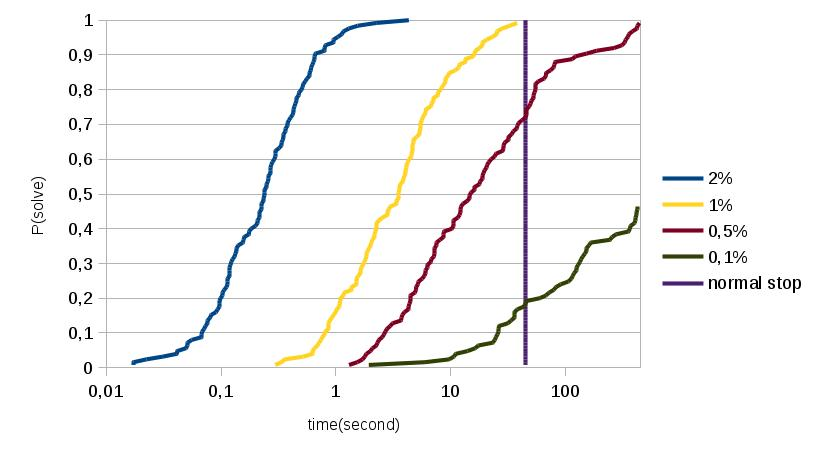
\includegraphics[scale=0.35]{Qualified_run_time_distribution.jpg}
\caption{Qualified run time distribution of ILS}
\label{Qualified run time distribution of ILS}
\end{figure}

\begin{figure}[!h]
\centering
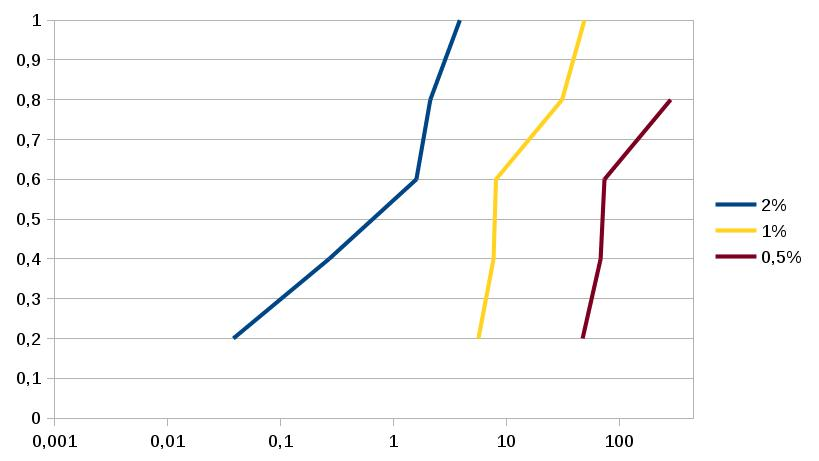
\includegraphics[scale=0.35]{Qualified_run_time_distribution2.jpg}
\caption{Qualified run time distribution of tabu}
\label{Qualified run time distribution of tabu}
\end{figure}

\begin{figure}[!h]
\centering
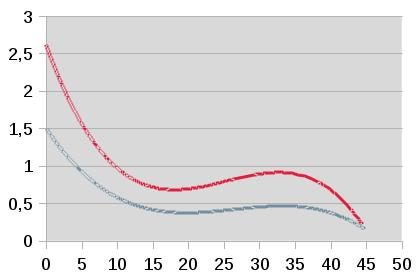
\includegraphics[scale=0.7]{corelation_plot_50.jpg}
\caption{Correlation plot on size 50 instances}
\label{Correlation plot on size 50 instances}
\end{figure}

\begin{figure}[!h]
\centering
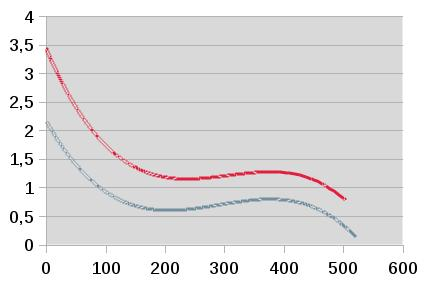
\includegraphics[scale=0.7]{corelation_plot_100.jpg}
\caption{Correlation plot on size 100 instances}
\label{Correlation plot on size 100 instances}
\end{figure}

Both correlation plot show the evolution of the average relative (in $\%$) deviation over the time (in second). They use the execution trace of one on each instances for both algorithm. The red line is for ILS and the blue one for tabuE. To have a smooth plot a polynomial regression of third degree had been used.

\section*{Conclusion}


\bibliographystyle{plain}
\bibliography{biblio}
\end{document}